The cooling trailer is an insulated trailer designed and built by Schmidt Cargobull with a cooling system developed by Termoking OR Carrier. It is attached to a truck and has a length of 13.4 meters. The trailer features room for 33 Euro-pallets of cargo and is used to transport various goods which need specific environmental conditions during transportation. The cooling system used to control the internal climate of the trailer is powered by a battery located in the trailer. This allows the trailer cooling to be powered independent of the truck.

While the trailer usually has its own cooling system made by Schmidt Cargobull, the trailer in this project utilizes a custom HVAC system designed by Bitzer. This system is built to facilitate testing of advanced control strategies.

The inputs and outputs of the system are the found by investigating the structure of the HVAC system. While the system will be described in detail in section XX, the most important components can be named as refrigerant moves around a loop through various components. These are: A scroll compressor, a condenser, a condenser throttle valve, a flash tank, an expansion valve and an evaporator. These can also be observed in \cref{fig_HVAC_Diagram}. The trailer box is also of great importance. 
The evaporator fan blows cold air throughout the top of the trailer, where it travels down past the cargo to the bottom and is pulled back along the floor.

\begin{figure}[h!]
	\centering
	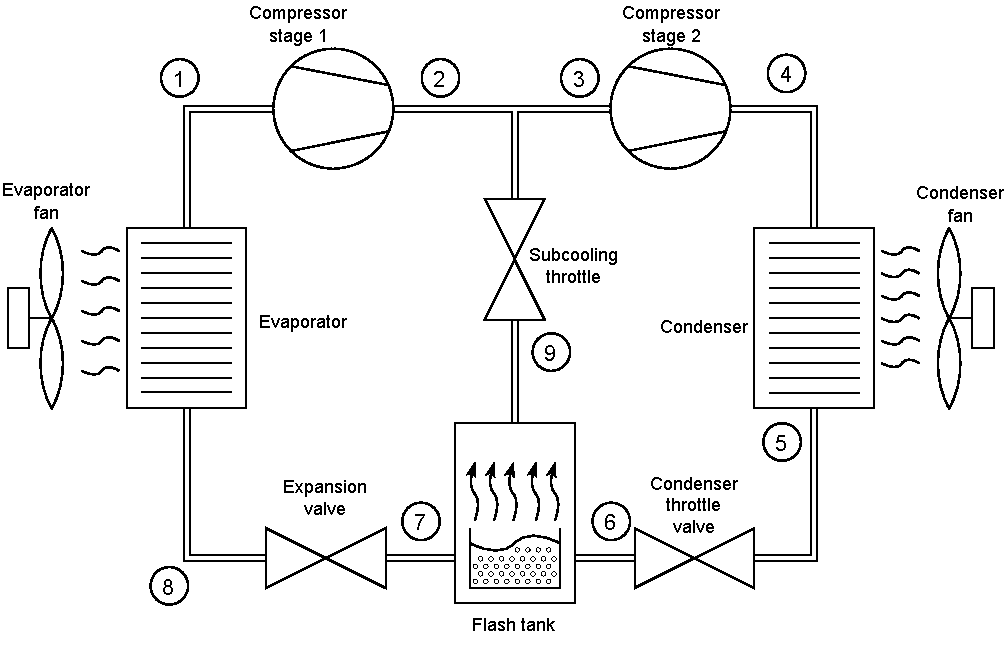
\includegraphics[width=0.85\textwidth]{Graphics/HVAC_Diagram_Fans.pdf}
	\caption{Illustration of refrigeration cycle}
	\label{fig:HVAC_Diagram}
\end{figure}

Many of the system components have variables that can be set to change their behavior. These are the controlled inputs, and include:

\begin{itemize}
	\item The compressor speed
	\item The condenser fan speed
	\item The evaporator fan speed
	\item The expansion valve opening degree (OD) to the evaporator
	\item The condenser throttling valve opening degree to the flash tank
\end{itemize}

There are many variables such as pressure and temperature throughout the refrigeration cycle, many of which are measured and hence are outputs of the system. 
The controlled outputs however, are those of interest from a control point of view. These are the outputs that the control strategy seeks to keep at a set point, in this project it will be the trailer box air temperature. The aim of the project is to design a Multiple-Inputs-Multiple-Outputs (MIMO) Controller to keep the temperature inside the container constant despite exogenous inputs (disturbances), specifically the ambient temperature. Furthermore it should do so with the sub-goal of minimizing the energy consumption.


In \cref{fig:p-h_diagram} a p-h diagram of the refrigeration cycle can be seen. It is not accurate but merely depicts the general idea of how the enthalpy and pressure changes throughout the cycle. The numbers in the figure are also shown in \cref{fig:HVAC_Diagram} for reference. Two cycles can be observed on the diagram. The first is the main cycle which runs along $1 \rightarrow 8$ and the second is the cycle running along $3\rightarrow 6 \rightarrow 9$.

\begin{figure}[h!]
	\centering
	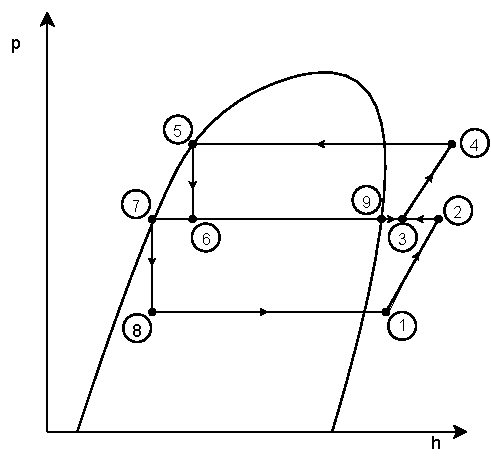
\includegraphics[width=0.55\textwidth]{Graphics/Flash_Tank_P-h_Diagram}
	\caption{P-h diagram of the refrigeration cycle}
	\label{fig:p-h_diagram}
\end{figure}




\subsection{What is it used for}


	
NOT DONE
Inputs / outputs

Control objectives
\begin{itemize}
	\item Constant temperature
		\begin{itemize}
			\item Disturbances
		\end{itemize}
	\item Minimum energy consumption
		\begin{itemize}
			\item Cost of batteries and prices of electricity
		\end{itemize}
\end{itemize}

		
